\documentclass[conference]{IEEEtran}
%\IEEEoverridecommandlockouts
% The preceding line is only needed to identify funding in the first footnote. If that is unneeded, please comment it out.
\usepackage{cite}
\usepackage{amsmath,amssymb,amsfonts}
%\newtheorem{Theorem}
%\newtheorem{Definition}
%\newtheorem{Lemma}
%\newtheorem{Proof}
\usepackage{algorithm}
\usepackage{algorithmic}
\usepackage{graphicx}  %for picture insert add by msc
\usepackage{float}
\usepackage{booktabs}  %for table line , add by msc
%\usepackage{cases}     %for equation , add by msc
\usepackage{textcomp}
\newtheorem{theorem}{\textbf{Theorem}}
\newtheorem{definition}{\textbf{Definition}}
\newtheorem{lemma}{\textbf{Lemma}}
\renewcommand{\algorithmicrequire}{\textbf{Input:}}  % Use Input in the format of Algorithm
\renewcommand{\algorithmicensure}{\textbf{Output:}} % Use Output in the format of Algorithm
%\usepackage[section]{placeins}
\def\BibTeX{{\rm B\kern-.05em{\sc i\kern-.025em b}\kern-.08em
    T\kern-.1667em\lower.7ex\hbox{E}\kern-.125emX}}


\begin{document}

\title{A Stochastic Network Calculus Approach for Delay Analysis of URLLC\\
%{\footnotesize \textsuperscript{*}Note: Sub-titles are not captured in Xplore and
%should not be used}
\thanks{Identify applicable funding agency here. If none, delete this.}
}
\title{A Stochastic Network Calculus Approach for URLLC delay analysis\\}
\title{Applying Stochastic Network Calculus Approach to delay analysis of URLLC \\}
\title{Analysis Delay Performance of URLLC Based on the Stochastic Network Calculus}
\title{Delay Analysis for URLLC in 5G Based on Stochastic Network Calculus\\}

\author{
%\IEEEauthorblockN{1\textsuperscript{st} Xin Chen}
%\IEEEauthorblockA{\textit{School of Computer Science} \\
%\textit{Beijing Information Science and Technology University}\\
%Beijing, China \\
%chenxin@bistu.edu.cn}
%\and
%\IEEEauthorblockN{2\textsuperscript{nd} Mark}
%\IEEEauthorblockA{\textit{School of Computer Science} \\
%\textit{Beijing Information Science and Technology University}\\
%Beijing, China \\
%mashengcheng@163.com}
%\and
%\IEEEauthorblockN{3\textsuperscript{rd} Zhuo Li}
%\IEEEauthorblockA{\textit{Beijing Key Laboratory of Internet Culture and Digital Dissemination Research} \\
%\textit{School of Computer Science} \\
%\textit{Beijing Information Science and Technology University}\\
%Beijing, China \\
%lizhuo@bistu.edu.cn}
}

\maketitle

\begin{abstract}
The fifth generation(5G) wireless networks are upcoming to our life. The higher performance requirements are raised to satisfy the needed in modern communication.
Ultra-reliable low-latency communications(URLLC) is one of the most importance scenarios in 5G. URLLC with strict requirements, especially in terms of latency and reliability, is widely used in some delay-sensitive applications such as self-driving.As the 3GPP claimed, the URLLC is amenable to 99.999\% transmission correctness and within 1ms delay bound.
How to meet the reliability and latency requirement is still a open issue. Some academic studies and companies proposed various methods to design URLLC standard, but little effort has been made on applying a theoretical method to limited the delay bound.
stochastic network calculus is an elegant way to obtain the delay bound based on traffic models and service guarantees.
In this paper, we use the stochastic network calculus to analysis the delay constraint in URLLC, which provide valuable guidelines for the early design of URLLC architecture.
In the end, numerical analyses are conducted to discuss the relationship between delay and the probability.
\end{abstract}

\begin{IEEEkeywords}
5G, URLLC, Stochastic Network Calculus, Delay Analysis
\end{IEEEkeywords}

\section{Introduction}
The 5G era is getting closer to us. 5G communication technology appeared for the first time with the 2018 Pyeongchang Winter Olympics where in South Korea. It helps audiences watch the live broadcast continuously and smoothly.
According to International Telecommunication Union announced the 5G standard timetable, 5G will start commercially in 2020 \cite{b1}.

The services with regard to next generation of mobile communication are in varied forms. These services have different requirements for the 5G networks. For example, industry automation requires low delay and high reliability, but the data rate is not high. High definition video does not require ultra reliable and low latency, yet need super high data rate. Some massive Internet of things ask for neither high speed nor low latency, whereas they need to support very high connection density simultaneously.

5G wireless networks are designed to support diverse and complicated scenarios which mentioned above.
The Third Generation Partnership Project(3GPP) classify these different scenarios into three big categories: enhanced mobile broadband(eMBB), massive machine type communications(mMTC), and ultra-reliable low-latency communications(URLLC) \cite{b2}.

URLLC is widely used in self-driving, mission critical application and some time delay sensitive systems.It has stringent requirements in terms of delay and reliability in the 5G New Radio(NR) systems. The key requirements of URLLC as claimed by the 3GPP are to ensure the latency of user plane data less than 1 ms for downlink and uplink, meanwhile to keep very high packet reception reliability, about 99.999 percent.\cite{b3}

So stringent delay requirement need new 5G NR technology to bridge the gap. Though the existing LTE networks can reach the reliability target, but the cost is some dozens of milliseconds time delay. That is far away from the criteria of URLLC. So the delay became the chock point and it need to be solved. Many academies and companies have proposed some engineering solutions to minimize the delay, like the HARQ retransmission or grant-free technology and so on. Whereas, how to analyze the generation of time-delay from a theoretical perspective and propose a group of tactics to reduce the delay effectively is an important research subject.

Stochastic network calculus(SNC) theory is very good at delay performance analysis. The SNC is a continuous development method to analysis network traffic characteristic and evaluate performance. The fundamental theory of SNC is network calculus, it was presented in the early 1990s. Network Stochastic has divided into two branches, deterministic network calculus and stochastic network calculus\cite{b4}. The deterministic network calculus system can provide minimize service guarantees by service curves\cite{b5}. But the deterministic model has the weakness that it can not utilize the statistical feature of traffic flow. To deal with random service and statistical guarantee, the SNC theory comes into being with a large number of stochastic processes and traffic models. Because of permitting some packets violates the desired performance, SNC can better take advantage of statistical multiplexing gains. Under a suitable traffic model and a chosen server model, The SNC theory can easily address delay, backlog and other service guarantee analysis of communication network. So we capitalize on the SNC method to build a model to simulate the 5G URLLC uplink and downlink transmission in this paper.

We use traffic-amount-centric stochastic arrival curve to describe the process that user equipment(UE) data sends to gNodeB side. It can be deduced the rest stages of data transmission from gNodeB to cloud server according to the 5G network topology architecture. Every stage of stochastic arrival curve characterizes the delay property, the whole delay of URLLC system is comprised by delays which generated from UE to cloud server.

Our main contributions of this paper can be summarized as follows:

1) We build a tandem model to simulate 5G network architecture. In this model we can analog the data transmission in uplink or downlink from UE to cloud server.

2) We use stochastic network calculus to analysis the delay bound.

3) Delay boundary has valuable theoretical guidance for the design of URLLC.

The rest of this paper is organized as follows. Section 2 summarizes related work of URLLC technology and stochastic network calculus. We present a stochastic network calculus model to describe URLLC  in Section 3. In particular, we illustrate the architecture of this system and explain . In section 4, we introduce the experimental environment and conduct the performance evaluation. We conclude this paper in Section 5.

\section{Related Work}

Because the standard of URLLC has not been worked out, many researchers have put forward different solutions for the design of URLLC.
%The architecture is depicted as Fig.\ref{fig_architecture}.
\begin{figure*}[htbp]
\centering
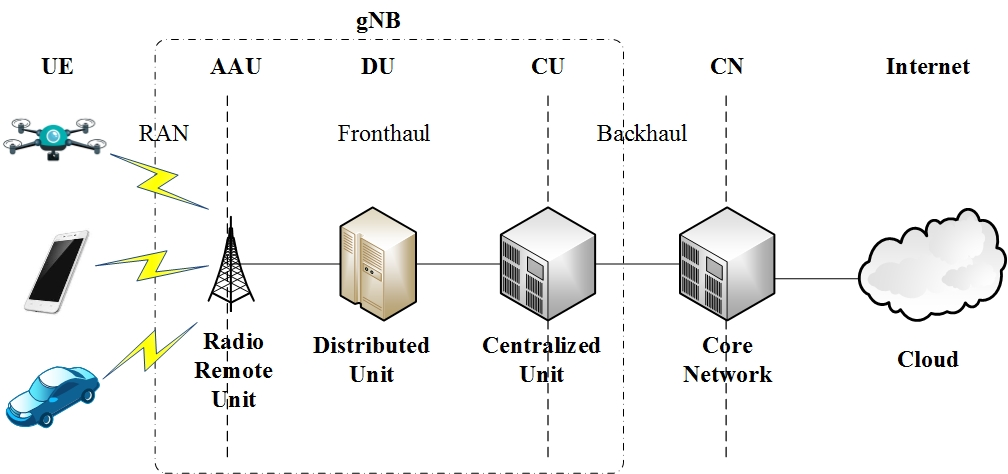
\includegraphics[width=.5\textwidth]{5G_delay_en.jpg}
\caption{5G network architecture.}
\label{fig_architecture}
\end{figure*}

There are many researches on how to implement URLLC and how to design it to meet the performance requirements of URLLC.
A way to offer URLLC without intervention in the baseband/PHY layer design is to use interface diversity and integrate multiple
communication interfaces. Jimmy and his colleagues propose an analysis framework that combines traditional reliability models with technology-specific latency probability distributions\cite{interface}. In this way, they can estimate the performance in terms of latency and reliability of such an integrated communication system.
To guarantee a low end-to-end delay with low jitter over combined internet and wireless interfaces, the article \cite{multiconnectivity} presents a new multiple-input multiple-output(MIMO) networked round trip time(RTT) skew control algorithm. This RRT skew controller's advantage is that the controller solves the data flow split problem at the controlling node, since the inner loop control signals are the downlink data rates that fully define the data flow split.
Jaya Rao and Sophie Vrzic have propose an approach to adopt packet duplication(PD) method to satisfy the latency and reliability requirements\cite{PD}. PD technology generates multiple instances and sends them simultaneously in multiple unrelated channels. The receiver selects the best packets according to the channel condition to achieve better transmission reliability. This PD technique can provide a cost-effective solution without increasing the complexity in the radio access network(RAN).

In terms of resource allocation and energy efficiency, there are also some researches on URLLC.
How frequency resource are allocated to send a user data in URLLC scenario? That is an interesting study which plunged by Anand A and De Veciana G\cite{Anand}. Based on the 5G standard technology Orthogonal Frequency Division Multiple Access (OFDMA), they build a One Shot Transmission model which does not allow retransmission.  Adopting queuing theory analysis, they find out a result that a small bandwidth over a longer duration is better than a large swath of bandwidth for short duration in One Shot Transmission system.
Green energy saving is getting more and more attention. The article \cite{Energy} provides a coordinated on-off switching scheme across a set of adjacent gNodeBs. The gNodeBs share a sleep schedule among themselves, where gNodeBs with lower offered traffic and fewer connected UEs select longer OFF durations. This is more energy-efficient with on-off mode than traditional mode on the premise of guaranteeing the time delay.

Because URLLC has strict requirements for delay and reliability, it is very meaningful to evaluate the performance of URLLC.
Joachim et al. provide an achievable latency bound evaluation in their article\cite{joachim}. They compare the worst case RAN transmission latencies for different 5G URLLC configurations. The configuration contains FDD, TDD, frequency numerologies and usage of slots. According the analysis, a frequency with higher numerology can be used to reduce the latency.
An article derived from HUAWEI propose a grant-free mode uplink transmission mechanism\cite{Huawei}. Grant-free transmission is a transmission without scheduling request and dynamic grant. This scheme is poised to meet the reliability requirement of URLLC in uplink transmission. By simulating different numbers of active UEs random arriving, the reliability can be improved after adopting the grant-free mode with increasing retransmission.

In order to satisfy the key requirements including latency and reliability, many state-of-the-art solutions have been discussed. These technologies contains fast HARQ retransmission, MIMO, beamforming, diversity interfaces, D2D communication, Ultra Density Network and so on \cite{Achieving}\cite{Wireless}\cite{Introduction}\cite{Physical}.
Some of these technologies can be employed alone to promote the performance, and others need to be combined together to achieve better results.
They all mentioned the design of frame structures. That because low latency and high reliability are contradictory. This requires more flexible frequency and time division.

Stochastic network calculus is a very practical tool, and has a good practical effect in performance analysis and theoretical boundary calculation.
At present, the most representative academic research teams are Yuming Jiang, Fidler M, Beijing University of Posts and Telecommunications(BUPT) and Beijing Information Science \& Technology University(BISTU). As shown in Table.\ref{tab_teams}.

\begin{table}[H]
\caption{Team that study SNC}\label{tab_teams}
\center
\begin{tabular}{ccc}
 \toprule
Team     & Research Types    & Research field \\
 \midrule
 Jiang   &Theory\&Application& Delay Evaluation\&Wireless \\
 Fidler M&   Theory          & Service Curve\&Estimation  \\
 BUPT    &   Application     &    Wireless communication  \\
 BISTU   &   Application     &    LTE\&Femtocells \\
 \bottomrule
\end{tabular}
\center
\end{table}

Yuming Jiang's research field is relatively extensive, including theory and application \cite{jiang_power}\cite{jiang_Delay}\cite{jiang_theory}\cite{jiang_Wireless}.
The research direction of Fidler M is more theoretical
\cite{MF_cross} \cite{MF_Service} \cite{MF_Estimation} \cite{MF_Random}.
BUPT and BISTU mostly adopt SNC to analyze performance criteria and quality of service in real networks.
The research field of BUPT is mainly in wireless network communication \cite{beiyou_1} \cite{beiyou_2} \cite{beiyou_lei1} \cite{beiyou_lei2}.
And the application background of BISTU is concentrated on the resource allocation and LTE networks
\cite{si_yuan}\cite{xiang_xd}\cite{xu_tong}\cite{zhang_lei}.

In these teams, there are often cooperation. The document \cite{MF_jiang} is an article of cooperation between Fidler M and Yuming Jiang, which mainly applies SNC theory to analyze the delay boundary of multi-server systems. Jiang also collaborate with BUPT team to evaluate the delay performance in wireless-powered communication system\cite{beiyou_1}.

%\FloatBarrier
\section{System Model}

\subsection{URLLC Network architecture}
We consider URLLC network as a concatenate system from UE to Cloud. We only consider the 5G standalone network situation.
The 4G LTE network is composed by UE, RRU(Radio Remote Unit), BBU(Building Base band Unit), the EPC(Evolved Packet Core) which is the LTE's core network, and end by cloud servers.

Different to the 4G LTE, 5G networks are composed by UE, gNB, CN and Cloud.
The gNB contains three parts that are AAU(Active Antenna Unit), DU(Distributed Unit) and CU(Centralized Unit).
AAU takes the place of the original RRU and combines some physical layer processing functions of BBU.
The BBU function of 4G will be rebuilt into DU and CU in 5G.
CU provides the service convergence function in the access side. It focuses on the low real-time capabilities of the protocol stack and adopt a centralized deployment.
DU mainly provides data access function to the terminal, including radio frequency and partial signal processing. DU concentrate on the high real-time capabilities of the transport requirements and suit for a distributed deployment method.
The CN(Core Network) in 5G replace the EPC. 5G CN is based on SDN/NFV technology and designed to better fit the cloud platform.
The architecture is depicted as Fig.\ref{fig_architecture}.

\subsection{Delay of URLLC Network}
UE devices firstly access to AAU. The AAU is actually a part of base station. This part of the communication belongs to RAN.
UE's data will be accepted by AAU, and AAU put forward the data to DU.
There are two situations when data arrive at DU.
If CU and DU are deployed together, the data can be CU immediately. Otherwise, the data will be sent to CU from DU.
The communication from AAU to CU belongs to fronthaul.
The data leave CU and continue upward to the CN. This part of the communication is called hackhaul.
CN will process the data and it will take some time.
Finally, CN will send the data to Cloud servers. The unidirectional transmission is finished.

So the whole delay or latency in 5G system is contribute by the time processing of RAN, fronthual, backhaul, CN and Cloud server. It can be expressed as Formula.\ref{eq_delay_composition}.
\begin{equation}\label{eq_delay_composition}
T_{Total} = T_{RAN} + T_{Fronthaul} + T_{Backhaul} + T_{CN} + T_{Cloud}
\end{equation}
where
\begin{itemize}
\item $T_{RAN}$ is the time cost by physical layer transmission between UEs and AAU.
\item $T_{Fronthaul}$ is the delay between AAU to CU. It is the time taken in gNB.
\item $T_{Backhaul}$ is the time taken to communication between gNB to CN.
\item $T_{CN}$ is the delay taken place in CN.
\item $T_{Cloud}$ is the latency which data transmission between CN and Cloud server.
\end{itemize}

To meet the URLLC key requirement, we should do a good job of studying $T_{Total}$.

In this part, we discuss the latency mainly on the User Plane(UP) rather than Control Plane(C-Plane). That because most of latency is attributed to the UP. UP latency is the communication time between network nodes and UE when transmission and reception of the data at the corresponding IP layer. Whereas, the C-Plane latency is the time spend on radio resource allocating and state switching from idle to active. Compared with UP latency, the C-Plane delay is tiny and can be ignored.

\subsection{Problem Description and Model Building}
The data transport from UEs and go through every nodes to cloud at the end.
according to the requirement of URLLC, the reliability and latency can be described as Formula.\ref{eq_urllc_problem}:

\begin{equation}\label{eq_urllc_problem}
P\{delay > \delta \} < \epsilon
\end{equation}

The delay should be within 1ms, so the $\delta < 1$, the unit is microsecond(ms). Where $epsilon$ is defined as a very small probability. Meanwhile the block error rate(BLER) must be 99.999\%. It means that the value of $\epsilon$ must be less than $1*10^{-5}$, (i.e. $1 - 1*10^{-5} = 0.99999$, It equals to BLER $99.999\%$). The Formula.\ref{eq_urllc_problem} represents the 5G URLLC network successfully transport data and satisfy the delay and reliability requirements.
%in here, I assume the ultra reliable and low latency in one formula, it may be not accurate.

\subsection{Stochastic Network Calculus}
In SNC theory, the min-plus algebra is applied to analyze queueing system. Let $\mathcal{F}$ denotes the set of non-negative non-decreasing functions and $\mathcal{\bar{F}}$ denotes the set of non-negative non-increasing function. We employ the cumulative process to represent amount of traffic flow. Arrival process, departure process and service process are denoted as $A(t)$, $D(t)$, and $S(t)$ respectively. For any $0 \leqslant s \leqslant t, A(0)=0, A(s,t) = A(t) - A(s)$, and practical significance of $A(t)$ is the cumulative arrival data at time $t$. It same to the $D(t)$ and $S(t)$. Some fundamental definitions of curve are well described in literature \cite{b4}, we utilize and expand the following in this paper.

\begin{definition}\label{def_SAC}
{\bfseries (Stochastic Arrival Curve)}. A flow is said to have a stochastic arrival curve $\alpha\in\mathcal{F}$ with bounding function $f\in\mathcal{\bar{F}}$, denoted by $A(t) \sim <f,\alpha>$, if for all $t \geq 0$ and all $x\geq0$ there holds
\begin{equation}\label{eq_sac}
P\Bigl\{\sup_{0\leq s \leq t}\{A(s,t) - \alpha(t-s)\} > x \Bigr\} \leq f(x).
\end{equation}
\end{definition}

where $\alpha(\tau)$ is the stochastic arrival curve, and it denotes the supremum of flow $A(\tau)$. Function $f(x)$ denotes the violation probability. It assumes that the stochastic arrival curve $\alpha(\tau)$ may be exceeded by arrival process $A(\tau)$ in sometimes, but the probability of being exceeded is constrained by the boundary function $f(x)$.

\begin{definition}\label{def_SSC}
{\bfseries(Stochastic Service Curve)}. A system $S$ is said to provide a stochastic service curve $\beta\in\mathcal{F}$ with bounding function $g \in \mathcal{\bar{F}}$, denoted by $S \sim<g, \beta>$, if for all $t\geq0$ there holds
\begin{equation}\label{eq_ssc}
P\Bigl\{\sup_{0\leq s \leq t}[A\otimes\beta(s) - D(s)] > x \Bigr\} \leq g(x).
\end{equation}
\end{definition}
%Current editing!

The operator/symbol $\otimes$ represents the cumulative min-plus convolution operation. Which
\begin{equation}\label{eq_convolution}
A\otimes\beta(t) = \inf_{0 \leqslant s \leqslant t}\{A(s)+\beta(s,t)\}
\end{equation}
$\beta(t)$ is the stochastic service curve which means the worst service capability provided by the server. Similar to the stochastic arrival curve, the data that already have been served are probably to be more than the leaving data. The probability of producing exceeding data can be constrained by the boundary function $g(x)$.

Similarly as in (\ref{eq_ssc}), the departure process can be related to the arrival and service process, for all $s,t \geqslant 0$ and $s \leqslant t$:
\begin{equation}\label{eq_departure}
D(t) = \inf_{0\leqslant s \leqslant t}\{A(s)+ S(s,t)\} =  A \otimes \beta(t).
\end{equation}
from the (\ref{eq_departure}), we can better understand the relationship among arrival process, departure process and service process. With these basic processes and curves, we can discuss the definition of the delay boundary.

\begin{definition}
{\bfseries(Latency Process)}.
Let $A(t)$ and $D(t)$ respectively be the arrival process and departure process. The latency process $L(t)$ at time $t \geq 0$ is defined as
\begin{equation}\label{eq_delay_define}
L(t) = \inf\{d \geq 0 : A(t) \leq D(t+d)\}.
\end{equation}
\end{definition}

The Formula.\ref{eq_delay_define} express that latency $L(t)$ is the least value of $d$, and the $d$ must meet the condition which the amount of arrival data at time $t$ is less than or equal to the departure data at time $t+d$. It also means that the data do not leave the server immediately. The duration of the data in server is the delay time. In Formula.\ref{eq_delay_define}, the arrival process $A(t)$ is little than or equal to the departure process $D(t+d)$. It means that the data arrived in server at time $t$ are all leave from server at time $t+d$. If $A(t)$ is large than or equal to the departure process $D(t+d)$, that represents the data arrived at $t$ moment have not been completed by service during $d$ period of time. So the $A(t)$ little than or equal to $D(t+d)$ situation is utilized to describe the shortest time that server takes for the data to be serviced. That is the latency or delay.

According to the latency process definition, and utilizing stochastic arrival process and stochastic service process, we have the result for stochastic latency bound.

%at this step, I should add the derivation process. Why the latency process will be like this.

\begin{theorem}{\bfseries (Stochastic Latency Bound)}
A system with an input process $A$. $A$ is a stochastic arrival process with stochastic arrival curve $\alpha \in \mathcal{F}$ and bounded by function $f \in \mathcal{\bar{F}}$ (i.e., $A \sim <f, \alpha>$). The system provides to the input a stochastic service process $S$. $S$ is with stochastic service curve $\beta \in \mathcal{F}$ with bounding function $g \in \mathcal{\bar{F}}$ (i.e., $S \sim <g, \beta>$). Then, for all $t\geq 0$ and $x \geq 0$, the Latency $L(t)$ is bounded by
\begin{equation}
P\{L(t)>h(\alpha+x, \beta)\}\leq f \otimes g(x)
\end{equation}
\end{theorem}
where function $h(\alpha+x, \beta)$ denotes the maximum horizontal distance between $\alpha+x$ and $\beta$, the express $f \otimes g(x)$ represents the cumulative min-plus convolution operation of function $f$ and $g$.

$Proof:$ Please see Appendix A.

\begin{theorem}{\bfseries (Concatenation Property)}
Consider a flow passing through a network of $N$ systems in tandem. If each system $n(=1,2,...,N)$ provides a stochastic service curve $S^{n}~<g^{n}, \beta^{n}>$ to its input, then the network guarantees to the flow a stochastic service curve $S~<g,\beta>$ with
\begin{align*}
\beta(t)=\beta^{1}\otimes\beta^{2}\otimes\cdot\cdot\cdot\otimes\beta^{N}(t) \\
\beta(x)=g^{1}\otimes g^{2}\otimes\cdot\cdot\cdot\otimes g^{N}(t)
\end{align*}
\end{theorem}
%here need to operation!

As assumption the latency of URLLC in Formula.\ref{eq_delay_composition},  We consider the URLLC network is a tandem system. So the delay of URLLC should fall in the concatenation characterization in SNC.

We consider that a UE's network flow passing through the gNB, CN and Cloud in tandem mode. Each network node $k(=gNB, AAU, DU, CU, CN, Cloud)$ provides a stochastic service curve $S_{k}\sim<g_k, \beta_k>$ to its flow, according to the concatenation property which mentioned in article \cite{b4}, then the network guarantees to the flow a stochastic service curve $S_{All}\sim<g_{All},\beta_{All}>$ with
\begin{equation}\label{eq_tandem_ssc}
\beta_{All}(t)=\beta_{gNB}\otimes\beta_{CN}\otimes\beta_{Cloud}(t)
\end{equation}
where
\begin{equation}\label{eq_tandem_gNB}
\beta_{gNB}(t)=\beta_{AAU}\otimes\beta_{DU}\otimes\beta_{CU}(t)
\end{equation}
actually
\begin{equation}\label{eq_tandem_sscFull}
\beta(t)_{All}=\beta_{AAU}\otimes\beta_{DU}\otimes\beta_{CU}\otimes\beta_{CN}\otimes\beta_{Cloud}(t)
\end{equation}
and
\begin{equation}\label{eq_tandem_ssc_bound}
g_{All}(x)=g_{gNB}\otimes g_{CN}\otimes g_{Cloud}(x)
\end{equation}
where
\begin{equation}\label{eq_tandem_gNB_bound}
g_{gNB}(x)=g_{AAU}\otimes g_{DU}\otimes g_{CU}(x)
\end{equation}
actually
\begin{equation}\label{eq_tandem_ssc_bound}
g_{All}(x)=g_{AAU}\otimes g_{DU}\otimes g_{CU}\otimes g_{CN}\otimes g_{Cloud}(x)
\end{equation}
so the delay of the URLLC system can be bounded by this.
\begin{equation}\label{eq_tandem_urllc_bound}
P\{L(x)>h(\alpha+x, \beta_{All})\} < f \otimes g_{All}(x)
\end{equation}


\section{Numerical and Performance Evaluation}

bounds are the target.
add some proof in the theory description.

Consider the URLLC system traffic arrival process and service process are both independent and stationary increments. the delay can be bounded by
\begin{equation}
P\{L(t)>d\} \leq E[e^{-\theta x}]
\end{equation}

We suppose $C$ denote amount of UEs in URLLC system, and $n$ is the index of UEs, which $n\in[1, C]$, let us denotes $l(n)$ as the data size in transmission. Each server in tandem system has the constant service rate. The Stochastic arrival process can be write as:
\begin{equation}
A(t)=\sum^{C}_{n=1}l(n)
\end{equation}


\subsection{Experimental Environment}
A general URLLC reliability requirement for one transmission of a packet is $1*-10^{-5}$ for 32 bytes with a user plane latency of 1ms.
Reliability = $1*-10^{-5}$, and user plane latency = $3^{-10}$ msec, for direct communication via sidelink and communication range of (e.g., a few meters)
Reliability = $1-10^{-5}$, and user plane latency = $3^{-10}$ msec, when the packet is relayed via BS.

\subsection{Performance Evaluation}
The target for mobility interruption time should be 0ms.
\section{Conclusions}

An Important Thing is that I should add the reference to the definition. To prove the definition's validity.

\section{Appendix}
Link level evaluation with deployment scenario specific operating point and system level simulation are to be performed for the evaluations of Indoor Hotspot, Urban Macro, Highway, and Urban grid for connected car.
For URLLC, the target for user plane latency should be 0.5ms for UL, and 0.5ms for DL
The target for control plane latency should be 10ms.

From the analysis and simulation results we can see that contention based grant-free transmission with resource shared by multiple users is more efficient than the grant-based or traditional transmission, and it can well meet the reliability requirement of URLLC within the latency bound.
\subsection{Appendix A}
$Proof:$ Since the latency process are defined as $L(t) = \inf\{d \geq 0 : A(t) \leq D(t+d)\}.$
event ${L(t)} > d$ implies event ${A(t)>D(t+d)}$, hence
\begin{equation}\label{eq_latency_bound1}
P\{L(t)>d\} \leqslant P\{{A(t)>D(t+d)}\} = P\{A(t) - D(t+d)> 0\}.
\end{equation}
Then we focus on the $\{A(t) - D(t+d)\}$ part. We put $A\otimes \beta(t+d)$ into (\ref{eq_latency_bound1}), we can get
\begin{align*}
&A(t) - D(t+d) \\
=&A(t) - A\otimes \beta(t+d) + A\otimes \beta(t+d) - D(t+d) \\
=&A(t) - \inf_{0\leqslant s \leqslant t+d}\{A(s)+ \beta(t+d-s)\} + A\otimes \beta(t+d) - D(t+d) \\
\leq &A(t-s) - \beta(t+d-s) + A\otimes \beta(t+d) - D(t+d) \\
\leq&A(t-s) - \alpha(t-s) + \alpha(t-s) - \beta(t+d-s) \\
&+A\otimes \beta(t+d) - D(t+d) \\
\leq &\sup_{0\leqslant s \leqslant t}\{A(t-s)-\alpha(t-s)\} \\
&+\alpha(t-s)-\beta(t+d-s) + A\otimes \beta(t+d)-D(t+d) \\
\leq &\sup_{0\leqslant s \leqslant t}\{A(t-s)-\alpha(t-s)\} \\
&+\{A\otimes \beta(t+d)-D(t+d)\}  \\
&+\alpha(t-s)-\beta(t+d-s) \\
\end{align*}
Based on the stochastic arrival curve (\ref{eq_sac}) and stochastic service curve analysis (\ref{eq_ssc}), we use $h(\alpha+x, \beta)$ replace the $d$. where $h(\alpha+x,\beta)$ is the maximum horizontal distance between $\alpha+x$ and $\beta$ for $x \geq 0$. The $h(\alpha,\beta)$ function implies the condition
\begin{equation}\label{condition}
\lim_{t\rightarrow\infty}[\alpha(t)-\beta(t)]\leq 0.
\end{equation}
we can obtain
\begin{align*}
P\{L(t)>h(\alpha+x, \beta)\} &\leqslant P\{\{A(t) - D(t+h(\alpha+x, \beta))\} > 0\}  \\
&\leqslant P\{\sup_{0\leqslant s \leqslant t}\{A(t-s)-\alpha(t-s)\}  \\
&+\sup_{0\leqslant s \leqslant t+h(\alpha+x, \beta)}\{A\otimes \beta(s)-D(s)\} \} \\
&\leqslant f(t)+g(x) \\
&\leqslant \inf\{f(t)+g(x-t)\} \\
&\leqslant f\otimes g(x)
\end{align*}

\section*{Acknowledgment}

This work was supported by these programs:

National Natural Science Foundation of China

(Nos.61370065,61502040),

National Key Technology Research and Development Program of the Ministry of Science and Technology of China

(No.2015BAK12B03-03),

Beijing Municipal Program for Excellent Teacher Promotion

(No.PXM2017\_014224.000028).

\begin{thebibliography}{00}
\bibitem{b1} ITU-R M.2083-0, “IMT Vision - Framework and Overall Objectives of the Future Development of IMT for 2020 and Beyond,” Sept 2015.
\bibitem{b2} 3GPP TR 38.913, “Study on Scenarios and Requirements for Next Generation Access Technologies,” June 2017.
\bibitem{b3} Soldani D, Guo Y J, Barani B, et al, “5G for Ultra-Reliable Low-Latency Communications,” IEEE Network, 2018, vol.32, no.2, pp.6-7.
\bibitem{b4} Jiang Y, Liu Y. “Stochastic Network Calculus,” Springer London, 2009.
\bibitem{b5} M. Fidler and A. Rizk, "A Guide to the Stochastic Network Calculus," in IEEE Communications Surveys \& Tutorials, vol. 17, no. 1, pp. 92-105, Firstquarter 2015. pp.92-105.
\bibitem{interface} J. J. Nielsen, R. Liu and P. Popovski, “Ultra-Reliable Low Latency Communication Using Interface Diversity,” IEEE Transactions on Communications, vol.66, no.3, pp.1322-1334, March 2018
\bibitem{multiconnectivity} Delgado R A, Lau K, Middleton R H, et al. “Networked Delay Control for 5G Wireless Machine-Type Communications Using Multiconnectivity,” IEEE Transactions on Control Systems Technology, vol.99, pp.1-16, 2018.
\bibitem{PD} Rao J, Vrzic S, “Packet Duplication for URLLC in 5G: Architectural Enhancements and Performance Analysis,” IEEE Network, vol.32, no.2, pp.32-40, 2018.
\bibitem{Anand} Anand A, De Veciana G, “Resource Allocation and HARQ Optimization for URLLC Traffic in 5G Wireless Networks,” 2018.
\bibitem{Energy} Mukherjee A, “Energy Efficiency and Delay in 5G Ultra-Reliable Low-Latency Communications System Architectures,” IEEE Network, 2018, 32(2):55-61.
\bibitem{joachim} Sachs J, Wikstrom G, Dudda T, et al, “5G Radio Network Design for Ultra-Reliable Low-Latency Communication,” IEEE Network, 2018, vol.32, no.2, pp.24-31.
\bibitem{Huawei} Wang C, Chen Y, Wu Y, et al. “Performance Evaluation of Grant-Free Transmission for Uplink URLLC Services,” IEEE, Vehicular Technology Conference: Vtc2017-Spring. IEEE, 2017:1-6.

\bibitem{Achieving} Pocovi G, Shariatmadari H, Berardinelli G, et al. “Achieving Ultra-Reliable Low-Latency Communications: Challenges and Envisioned System Enhancements,” IEEE Network, vol.32, no.2, pp.8-15, 2018.
\bibitem{Wireless} Popovski P, Nielsen J J, Stefanovic C, et al. Wireless Access for Ultra-Reliable Low-Latency Communication: Principles and Building Blocks[J]. IEEE Network, 2018, 32(2):16-23.
\bibitem{Introduction} Ji H, Park S, Yeo J, et al. Introduction to Ultra Reliable and Low Latency Communications in 5G[J]. 2017.
\bibitem{Physical} Ji H, Park S, Yeo J, et al. Ultra Reliable and Low Latency Communications in 5G Downlink: Physical Layer Aspects[J]. 2018.

%jiang
\bibitem{jiang_power} Z. Li, Y. Jiang, Y. Gao, P. Li, L. Sang and D. Yang, "Delay and Delay-Constrained Throughput Performance of a Wireless-Powered Communication System," in IEEE Access, vol. 5, pp. 21620-21631, 2017.
\bibitem{jiang_Wireless} Sun F, Li L, Jiang Y. Impact of duty cycle on end-to-end performance in a Wireless Sensor Network[C]// Wireless Communications and NETWORKING Conference. IEEE, 2015:1906-1911.
\bibitem{jiang_theory} Jiang Y. Network calculus and queueing theory: two sides of one coin: invited paper[C]// International ICST Conference on PERFORMANCE Evaluation Methodologies \& TOOLS. 2014.
\bibitem{jiang_Delay} Mahmood K, Vehkaper M, Jiang Y. Delay constrained throughput analysis of SISO[C]// IEEE International Conference on Network Infrastructure and Digital Content. IEEE, 2013:116-121.

%M Fidler
\bibitem{MF_cross} S. Akin and M. Fidler, "A Method for Cross-Layer Analysis of Transmit Buffer Delays in Message Index Domain," in IEEE Transactions on Vehicular Technology, vol. 67, no. 3, pp. 2698-2712, March 2018.
\bibitem{MF_Service} R. Lübben and M. Fidler, "Service Curve Estimation-Based Characterization and Evaluation of Closed-Loop Flow Control," in IEEE Transactions on Network and Service Management, vol. 14, no. 1, pp. 161-175, March 2017.
\bibitem{MF_Estimation} R. Lübben and M. Fidler, "Estimation method for the delay performance of closed-loop flow control with application to TCP," IEEE INFOCOM 2016 - The 35th Annual IEEE International Conference on Computer Communications, San Francisco, CA, 2016, pp. 1-9.
\bibitem{MF_Random} R. Lübben, M. Fidler and J. Liebeherr, "Stochastic Bandwidth Estimation in Networks With Random Service," in IEEE/ACM Transactions on Networking, vol. 22, no. 2, pp. 484-497, April 2014.

%BUPT
\bibitem{beiyou_1} Z. Li, Y. Jiang, Y. Gao, P. Li, L. Sang and D. Yang, "Delay and Delay-Constrained Throughput Performance of a Wireless-Powered Communication System," in IEEE Access, vol. 5, pp. 21620-21631, 2017.
\bibitem{beiyou_2} Z. Li, Y. Gao, B. A. Salihu, et al, “Network Calculus Delay Bounds in Multi-Server Queueing Networks with Stochastic Arrivals and Stochastic Services”, IEEE Global Communications Conference. IEEE, 2015:1-7.
\bibitem{beiyou_lei1} K. Zheng, F. Liu, L. Lei, C. Lin and Y. Jiang, "Stochastic Performance Analysis of a Wireless Finite-State Markov Channel," in IEEE Transactions on Wireless Communications, vol. 12, no. 2, pp. 782-793, February 2013.
\bibitem{beiyou_lei2} Y. Li, L. Lei, Z. Zhong and S. Lin, "Performance analysis for high-speed railway communication network using stochastic network calculus," 5th IET International Conference on Wireless, Mobile and Multimedia Networks (ICWMMN 2013), Beijing, 2013, pp. 100-105.

%BISTU
\bibitem{si_yuan} Chen, Xin, Y. Si, and X. Xiang. Delay-bounded resource allocation for femtocells exploiting the statistical multiplexing gain. Kluwer Academic Publishers, 2015.
\bibitem{xiang_xd} X. Chen, Y. Si and X. Xiang, "Delay-bounded priority-driven resource allocation for two-tier macrocell/femtocell downlink," The 2014 5th International Conference on Game Theory for Networks, Beijing, 2014, pp. 1-6.
\bibitem{xu_tong} Tong Xu, Xin Chen, Xudong Xiang and Jianxiong Wan, "Delay analysis for cognitive radio networks with parallel Markov modulated on-off channels," ISWPC 2012 proceedings, Dalian, 2012, pp. 1-5.
\bibitem{zhang_lei} Lei Zhang, Xin Chen, Xudong Xiang and Jianxiong Wan, "A stochastic network calculus approach for the end-to-end delay analysis of LTE networks," 2011 International Conference on Selected Topics in Mobile and Wireless Networking (iCOST), Shanghai, 2011, pp. 30-35.

%cooperation
\bibitem{MF_jiang} M. Fidler, B. Walker and Y. Jiang, "Non-Asymptotic Delay Bounds for Multi-Server Systems with Synchronization Constraints," in IEEE Transactions on Parallel and Distributed Systems, vol. 29, no. 7, pp. 1545-1559, July 1 2018.


\end{thebibliography}

\end{document}
